%% Copernicus Publications Manuscript Preparation Template for LaTeX Submissions
%% ---------------------------------
%% This template should be used for copernicus.cls
%% The class file and some style files are bundled in the Copernicus Latex Package, which can be downloaded from the different journal webpages.
%% For further assistance please contact Copernicus Publications at: production@copernicus.org
%% https://publications.copernicus.org/for_authors/manuscript_preparation.html


%% Please use the following documentclass and journal abbreviations for preprints and final revised papers.

%% 2-column papers and preprints
\documentclass[tc, manuscript]{copernicus}

\usepackage{placeins}



\begin{document}

\title{Response to Reviewer 2 for "Snow accumulation variability limits InSAR SWE retrieval"}


% \Author[affil]{given_name}{surname}

\Author[1][zmhoppinen@alaska.edu]{Zachary}{Hoppinen} %% correspondence author
\Author[1]{Simon}{Zwieback}
\Author[2]{Ross}{Palomaki}
\Author[3]{Hans-Peter}{Marshall}

\affil[1]{Geophysical Institute, University of Alaska Fairbanks, 2156 Koyukuk Drive, Fairbanks, AK}

% \affil[1]{Institute of Arctic and Alpine Research, University of Colorado, 4001 Discovery Dr, Boulder, CO 80303, USA}
\affil[2]{Institute of Arctic and Alpine Research, University of Colorado, 4001 Discovery Dr, Boulder, CO 80303, USA}
\affil[3]{Department of Geosciences, Boise State University, 1910 University Drive, Boise, ID 83725, USA}

\runningauthor{Z. Hoppinen et al.}
\runningtitle{Response to Reviewer 2}
\maketitle

\textbf{General Comments:}

\textit{Thanks to the authors for this contribution. The idea presented is relatively new to the dInSAR
technique for dSWE and it presents interesting discussion on multilooking window selection
for processing. However, I have found issues that prevent me from recommending its
publication without a major revision. The paper needs to broaden theoretical discussion,
including selected references and provide a more thoughtful discussion on their findings.}

Thank you for taking time to read and give this thoughtful review. We agree with almost all of your points and think the text is much clearer for your comments. All line, figure, and section numbering refer to the revised version.

\textit{There are important papers that should be consulted as they discuss coherence for nonstationary processes. Touzi et al., 1999 models differently the non-stationarity. Yueh et al., 2026 directly addresses the topic presented here. The latter is particularly important here. Also consider Rott et al., 2003, although the formulation is for sub-pixel scale.} 

Thank you. All three are now cited, together with Zebker and Chen (2005), which treats the same estimation problem: Rott et al. (2003) and Yueh et al. (2026) in the introduction and Section~2.1 as the Gaussian analytic treatments whose result is the first term of our expansion, Touzi et al. (1999) and Zebker and Chen (2005) in Sections~2 and 3.6 for the stationarity requirement and the two competing biases (lines 60, 86, 106, 134, and 238).

\textit{An important addition to the paper would be to quantify both the absolute value and the argument of M with respect to standard deviation or relevant metrics within the window. Now, the reader cannot quantify the any impact of the variability. It is necessary to better quantify the magnitude of the effect. Consider the following:}
\begin{itemize}
    \item \textit{Choose a window size and generate phase samples (“per-cell deviation from mean”)}
    \item \textit{Calculate complex M, repeat enough times till convergence.}
    \item \textit{Repeat for different values of sigma. This would provide an idea of the effect of M for different window variabilities, instead of the arbitrary examples presented in Figure 1.}
\end{itemize}
\textit{This can also be calculated analytically but of course it's more tedious. Consider this both in absolute dSWE and radians. Consider different distributions. For example, in case the underlying distribution is Gaussian of $\delta$ or a symmetric distribution in general, I would expect that E{arg(M)} = 0. This is your case in Figure 1 (middle). Then, the estimated phase from the window will not be skewed. The reader needs to understand already in section 2 what causes the skewing.}

\textit{How does the typical multilooking window look like in terms of ΔSWE Which distribution approximate it better? This could be linked to your dataset. Based on your results (Figure 5), the distribution of ΔSWE may not be symmetrical. While this is partially addressed in Section 4.2, I think the aggregation over the whole dataset does not allow understanding of the individual multilook variability.}

We agree that the reader needs a number. Section~2.1 now expands $\log M$ in the cumulants of the within-window phase distribution, giving $|M|$ and $\arg(M)$ to leading order (Eqs.~7 and 8), and Figure~7 in Section~4.2 plots both against the phase spread over all lidar windows. The first term is the Gaussian result of Rott et al. (2003) and Yueh et al. (2026). The second is the bias, which a Gaussian cannot produce and which the odd moments cause. We do use the lidar windows as the background of Figure~7 in addition to your theoretical suggestion, as we feel that grounding the results in the actual observed $\Delta$SWE values is useful. Figure~7 shows every window individually rather than an aggregate. We have not fitted a named distribution, because beyond about 1.5\,rad of spread the phase wraps and $M$ depends on the full shape of the distribution rather than on any low-order family.

\textit{Another important consideration are variations of local incidence angle in the multilooking window. Although the sensitivity is smaller than ΔSWE changes in LIA within the multilooking window will produce the same effect even for constant ΔSWE In particular to your dataset, the northeast area seems to have lower values of M, but also presents more topographical variations.}

We use a constant local incidence angle of 40$^\circ$ (Section 3.4) over the lidar extent for the ASO-based conversions, so this is not a factor in our results, and the low $|M|$ in the northeast of the basin is $\Delta$SWE structure rather than terrain geometry. We have added a sentence to Section 3.4 to clarify this and a sentence to the Limitations about the potential for local incidence angle variations to add to or reduce the within-window effects over real terrain. The NISAR analysis, since it compares the storm pair against the no-accumulation pair, holds the local incidence angle constant in that part of the comparison, though the larger spread of incidence angle within an 80\,m window than within a 20\,m window might affect it.

\textit{Can you report the spatial baseline between NISAR acquisitions? The orbital tube for NISAR is small, but I wonder if small spatial baseline between passes can impact the coherence in some areas of your images.}

The perpendicular baselines, read from the GUNW metadata over the lidar extent, are $-109$\,m (range $-111$ to $-106$\,m) for December 7--19 and $127$\,m (123 to 131\,m) for December 19--31, with parallel baselines of $-69$ and $105$\,m. At the basin's 44.7$^\circ$ incidence angle and 1009\,km slant range these give heights of ambiguity of 790\,m (700 to 880\,m) and 680\,m (600 to 760\,m). The critical baseline for the 40\,MHz range bandwidth is 27\,km at the 40$^\circ$ local incidence angle used in the analysis (32\,km at the basin's 44.7$^\circ$ metadata incidence on flat terrain), so the geometric (spatial) decorrelation is 0.004 to 0.005 for both pairs. For a slope facing the radar at a 10$^\circ$ local incidence angle it rises to about 0.02. Spatial decorrelation is therefore negligible. Section 3.1 now states the baselines and heights of ambiguity (line 151).

\textit{A distinction between posting, resolution and multilook is needed. The multilooked domain, either 5x6 or 13x16, does not correspond to 20 or 81 ground meters, as multilooking is calculated in radar coordinates. Range resolution also depends with incidence angle. Comparing NISAR coherence and Lidar-derived M needs to be done with care (e.g., Section 4.3).}

We agree, and we have made the distinction explicit and standardized the wording. Section 3.4 now states this nuance where the lidar window sizes are chosen, and says that the square 81 and 21\,m lidar windows are close proxies for the two NISAR windows and that the analysis addresses the multi-look window on the snow side rather than reproducing the NISAR geocoding (lines 212--215). Throughout the manuscript we now use ``window'' and ``window size'' for the averaging block, ``posting'' for the 20 and 80\,m GUNW grids and ``resolution'' for the single-look cell and the ASO products, and have removed ``footprint'' and ``multi-resolution'', including from the section titles of Sections 3.6 and 4.4. We think this change was a great suggestion that really clarifies the text especially combined with the new Figure~1 suggested by reviewer 1.

\textit{The terminology “within-window”, “sub-window”, and “footprint” is used somewhat interchangeably throughout the manuscript.}

We agree this was confusing for a reader. See above comment where we also remove footprint. We have also standardized to within-window and removed sub-window throughout.

\textbf{Specific Comments:}


\textit{The abstract and introduction does not stress enough the main problem. Phase is highly sensitive to ΔSWE and ΔSWEis highly spatially variable. Also high decorrelation makes large multilooking an attractive option to deal with noise at a cost of spatial resolution.}

We agree. The introduction now states the phase sensitivity after Eq.~(1) and opens the deformation-gradient paragraph with why retrievals multi-look and what that assumes (lines 37--38 and 46--52). The spatial variability of $\Delta$SWE was already stated (lines 39--40).


\textit{Section 2: Somewhere along the first paragraph it should be commented that this “averaging” is performed spatially.}

We updated text in the first paragraph and new figures to clarify what is meant by averaging, and that it is performed spatially.

\textit{Equation 2 should be introduced more clearly.}

The lead-in to Eq.~(2) now says why the phase is decomposed and defines $\delta$ as the difference from the window mean (lines 90--94). The $\phi = \Delta\phi$ shorthand has been removed and $\Delta\phi$ is used throughout.

\textit{Figure 1 requires more explanation, describe how many pixels are you using, the central frequency you are using (as later described this is critical). Also consider discussing if the presented dynamic range is reasonable for SAR revisit times. Do you observe ±8cm=80mm ΔSWE often?}

This is an illustration of the effects we discuss later. The three panels and their values are chosen to isolate the constant, symmetric, and skewed cases synthetically, not observations, and we have kept the figure free of data detail for that reason. The caption now states that each window holds 12$\times$12 cells and that the phasors use the L-band $\kappa$ of Section~3.4 (52.7\,rad\,m$^{-1}$ at 40$^\circ$). The $\pm8$\,cm range is large but realistic for these pairs: the within-window standard deviation of $\Delta$SWE at 81\,m has a median of 3.4\,cm and a 1st to 99th percentile range of 0.9 to 23\,cm, so cells differing by 8\,cm within one window are possible, and the basin-median $\Delta$SWE of the largest event is 23\,cm. The figure is also clearer to the reader for having a larger spread.

\textit{ I think you need to differentiate between real noise free ΔSWE or Δ$\phi$ and observed values. For example, in Line 86 it is unclear if $\delta$ refers to stochastic noise or ΔSWE deviations from the mean. If the process is stationary, then $\delta$ = 0 for every pixel. The section already discusses in terms of estimated phase variance when in my understanding, you are discussing the effect of the underlying distribution of ΔSWE}

Agreed, $\delta$ was used for two things. The paragraph after Eq.~(4) is rewritten so that Eqs.~(2) to (4) are noise-free, $\delta$ is the $\Delta$SWE deviation only, and decorrelation noise stays in $\gamma_\mathrm{other}$. The lead-ins to Eqs.~(3) and (6) no longer say ``observed'' (lines 102--103, with the lead-ins at lines 95 and 122).

\textit{Section 3.4: When using the LIA=40 for the whole image, the topography is ignored, which varies subwindow variability.}

Agreed. As noted in our reply to the general comment above, the constant 40$^\circ$ incidence angle means the reported $|M|$ and $\arg(M)$ isolate the $\Delta$SWE variability alone, which Section 3.4 now states (line 205). The new Limitations paragraph quantifies what within-window variation of the local incidence angle over real terrain would add and notes that the within-window loss over steep terrain may be somewhat smaller or larger than reported (lines 517--522).

\textit{Section 3.6: The claim on the Circular Gaussian as the limitation is unclear.}

The sentence now says what the assumption is, fully developed speckle from many independent scatterers per cell, and that cells with only a few strong scatterers depart from it, where the bias correction is only approximate (lines 249--250).

\textit{Equation 8 is based on stationary samples. Since the central discussion of the paper is the non-stationarity I think commenting the validity of this equation is in order.}

Agreed that Eq.~(11) assumes looks that share one coherence and one phase. We apply it as if each window had the effective coherence $|M|\gamma_\mathrm{other}$, with $M$ the mean phasor of that window's own cells. We checked this by simulation (stats/plot\_bamler\_nonstationary.py in the repository), drawing looks from the same speckle model Eq.~(11) assumes but giving each window its own within-window phase pattern. Figure~\ref{fig:resp_bamler} shows that the de-biased sample coherence tracks the window's true $|M|\gamma_\mathrm{other}$ closely at both look counts, across the range of coherence and spread relevant here, while the raw sample coherence sits above it. We have kept this in the reply rather than the main text, where Section~3.6 is already dense, but would add a sentence there if the referee prefers.

\begin{figure}[h]
    \centering
    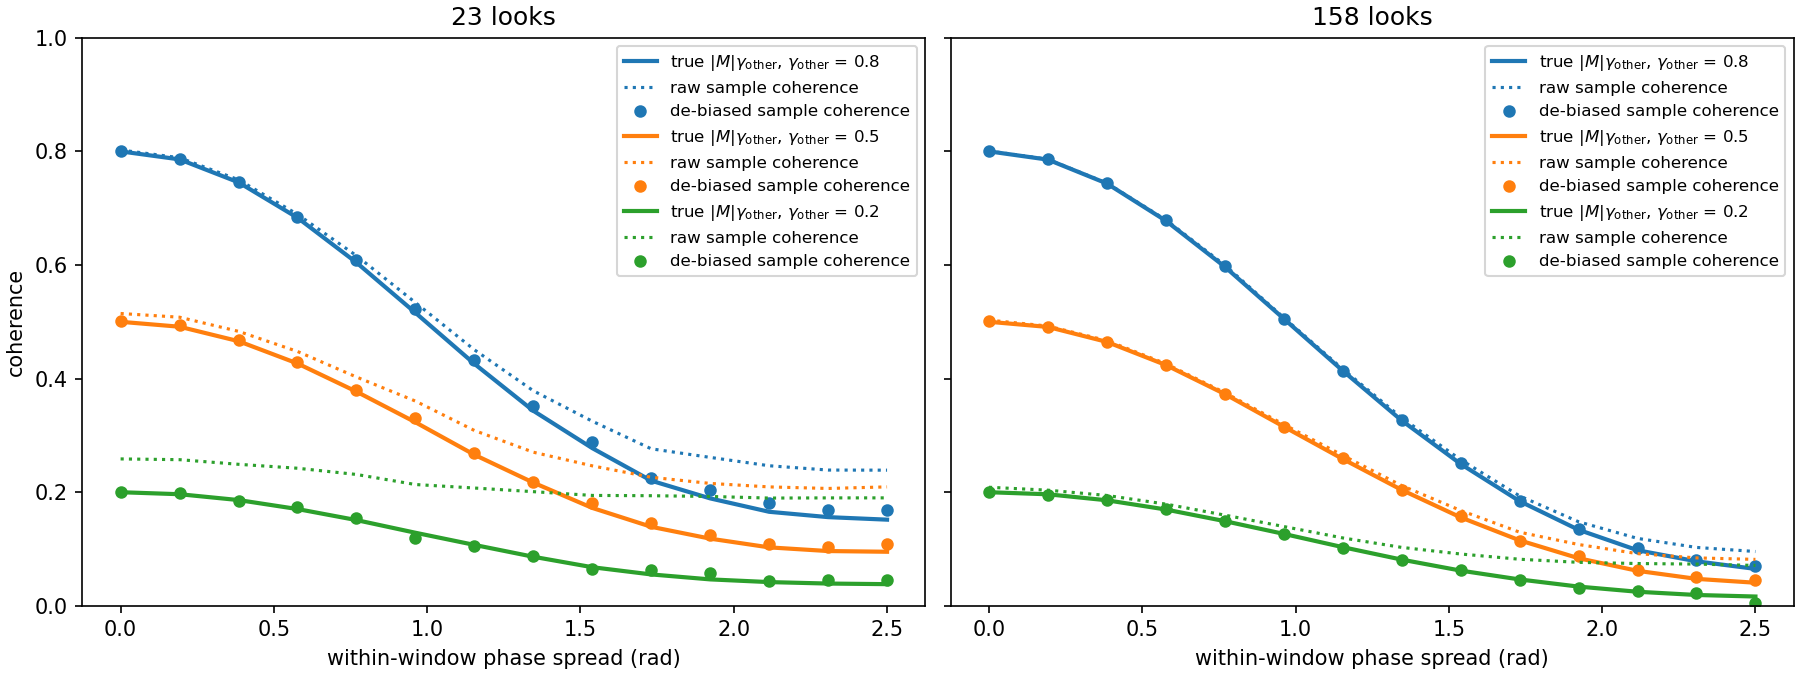
\includegraphics[width=1.0\linewidth]{figures/response_bamler_nonstationary.png}
    \caption{True effective coherence of each window, $|M|\gamma_\mathrm{other}$ with $M$ the mean phasor of its own cells (solid), raw mean sample coherence (dotted), and Bamler-de-biased sample coherence (markers) against the within-window phase spread, for 23 looks (\textbf{left}) and 158 looks (\textbf{right}) and $\gamma_\mathrm{other}$ of 0.8, 0.5, and 0.2. Monte Carlo over 3000 windows per point, each with its own Gaussian phase pattern.}
    \label{fig:resp_bamler}
\end{figure}

\textit{Section 4.5: The results, in particular related to C-band are quite pessimistic. How do these compare to literature, for example Oveisgharan et al., 2024, Oveisgharan et al., 2026, Bovenga et al., 2025 among others? This requires reconciliation with previous papers.}

The C-band result is pessimistic for large events, and we think that is likely an accurate estimate of C-band ability to resolve these large events. Eq.~(8) shows this: C-band keeps a coherence factor above 0.3 only where the within-window $\Delta$SWE spread is below about 0.7\,cm, whereas the Tuolumne storm windows have a median spread of 3.4\,cm. The C-band retrievals of Oveisgharan et al. (2024, 2026) and Bovenga et al. (2025) were made in snow climates with smaller accumulations, where that condition might be met, and our Limitations describe the Tuolumne storm pairs as an upper bound. For major accumulation events in complex terrain, our result implies that within-window variability would probably prevent a C-band retrieval, which calls for testing with lidar pairs in the basins where C-band has been applied. Section~5.4 now states this and lists that test as important future work (lines 455--458).

\textit{Section 5.2: I don't agree with this. For tower imagery I would not expect high spatial variability within the multilook window. The whole window may be smaller than a typical satellite resolution cell.}

Agreed. SodSAR images 0.1\,m pixels over a scene of about 35 by 30\,m (Ruiz et al., 2020), below a single satellite resolution cell, so its wind dependence is not evidence for variation between cells across a multi-look window. The paragraph no longer claims that, and now places the tower result at the sub-cell scale of Rott et al. (2003) (lines 417--418).

\textit{Snow depth/SWE for sea ice snow, is typically smaller than land. This is hinted on line 433. This is why I believe you need to quantify either analytically or numerically the effect of phase variance in the complex coherence.}

Agreed on both points. The quantification is now Eq.~(8) and Figure~7: the coherence loss is set by the within-window phase spread, $|M| \approx e^{-\kappa^2\sigma_{\Delta\mathrm{SWE}}^2/2}$, and the bias by its skew. The smaller snow depth and $\Delta$SWE over sea ice enter directly through $\sigma_{\Delta\mathrm{SWE}}$, so for the same wavelength and window a sea-ice snowpack with a few centimeters of accumulation and a small within-window spread sits far up the curve of Figure~7 where the Gaussian term holds and the bias is negligible, whereas the Tuolumne storm windows, with a median spread of 3.4\,cm, sit past the wrap limit at C-band. Our reference to Ming et al. (2026) is to the mechanism they identify, not to the magnitude, which Eq.~(8) shows must be smaller over sea ice.

\textbf{Specific Comments:}

\textit{Line 22: how “approximately weekly observations” are meet? Which constellation? S1? Where?}

The weekly figure refers to NISAR. Each track repeats every 12 days, but most locations lie in the overlap of ascending and descending tracks, and often of adjacent tracks, so a given location is imaged several times per 12-day cycle.

\textit{Line 48 to 50: These two sentences discusses different issues, variability in the pixel and within the estimation window, and are provided without reference.}

The two sentences are now one paragraph that introduces multi-looking, the constant-$\Delta$SWE assumption it makes, and the coherence loss and bias that within-window variability produces (lines 46--52). We have removed the Massonnet and Feigl (1998) gradient sentence from it. After adding the references suggested above, Rott et al. (2003), Yueh et al. (2026), Touzi et al. (1999), and Zebker and Chen (2005), we felt it added little, and cut it to keep the focus on those studies.

\textit{Line 50: Not completely sure if the original quote refers to your problem or phase unwrapping errors, as differences larger than 2pi cannot be recovered with some unwrapping tools.}

The quoted limit was the coherence one, derived in Massonnet and Feigl (1998, section 1.3.2, ``Gradient'') from the necessary condition for interferometry rather than from unwrapping, but as noted in the reply above we have removed the sentence from the manuscript.

\textit{Line 74: PDF require definition?}

It was the only use of the abbreviation, so we have replaced it with ``phase distribution'' (line 105).

\textit{Line 86: I would suppose that all terms in this section are already noise-free, then how is $\delta$ decorrelation noise alone?}

They are, and the sentence was wrong. As described in our reply to the Section~2 comment above, the paragraph after Eq.~(4) is rewritten so that $\delta$ is the noise-free $\Delta$SWE deviation only and decorrelation noise is kept in $\gamma_\mathrm{other}$ (lines 102--103).

\textit{Line 102: This is repeated.}

Removed. The unit-amplitude assumption is stated where Eq.~(3) is introduced and its consequences are discussed in the Limitations, so the repetition after the Figure~2 discussion is gone (line 95).

\textit{Line 103: not necessarily true for all frequencies.}

Agreed. The sentence now restricts the independence, and the multiplicative form of Eq.~(5), to L-band and longer wavelengths, and says why (lines 116--120).

\textit{Line 164: Int.phase is defined between (-pi, pi].}

Corrected to $(-\pi, \pi]$ (line 203). The one other occurrence, in Section 3.5, already used the half-open interval.

\textit{Line 328 and 333: Again the effect of the LIA could be affecting the non-stationarity.}

The incidence angle can affect the NISAR windows, unlike the lidar analysis where it is held fixed, but its sign is not determined. The cell phase is $\kappa(\theta)\,\Delta$SWE, so within-window variation of the local incidence angle adds to the spread where deeper accumulation coincides with larger $\kappa$ and partly cancels it where the two are anticorrelated, as the Limitations paragraph states (lines 517--522). The no-accumulation pair shows that terrain geometry alone does not produce the residual. Which way the incidence-angle term acted over the December storm cannot be resolved without a lidar pair coincident with the NISAR dates, which we list as the clearest next step (Section~5.5).

\textit{Line 342: I don't agree with this, see my points regarding Section 2.}

We have softened this. The sentence now says those areas may not be recoverable at the window sizes of current spaceborne products, rather than at any window size, and grounds it in the window-size sweep (line 408).

\textit{Line 406: I think those paper start my [by] calculating coherence spatially, so I don't think saying they use temporal rather than spatial averaging is right, can you check?}

Correct, and the sentence was wrong. We were using the main text's averaging language to draw the connection and went too far. Phase linking still forms the coherence spatially but can use smaller spatial windows because of the redundancy of the stack's pairs, which the sentence now says (lines 476--477).

\textit{Line 412: drop the formula of the phase closure as neither it or z are defined or used elsewhere.}

Dropped. The sentence now describes the closure phase in words, as the sum of the interferometric phases around a triplet of acquisitions (line 480).

\textit{Figure 7 refers to sub-pixel on the title.}

Corrected. The figure title now reads ``WY2025 (17 days): M by band at 81 m'' (now Figure~10), and ``sub-pixel'' does not appear anywhere in the manuscript.


\end{document}